\subsection*{Background theory}
The stream function is a function of coordinates and time of an inviscid liquid.
It allows to determine the components of velocity by differentiating the stream function 
with respect to the space coordinates. 
A family of curves $\Psi = const$ represent {\it streamlines}, i.e. 
the stream function remains constant along a streamline. 
Although also valid in 3D, this approach is mostly used in 2D because of its 
relative simplicity {\color{red} REFERENCES}.

In two dimensions the velocity is obtained as follows:
\begin{equation}
{\bm v} = \left( \frac{\partial \Psi}{\partial y},-\frac{\partial \Psi}{\partial x} \right) 
\end{equation}
Provided the function $\Psi$ is a smooth enough function, 
this automatically insures that the flow is incompressible:
\begin{equation}
{\bm \nabla}\cdot {\bm v} = 
\frac{\partial u}{\partial x} + \frac{\partial v}{\partial y}
=
\frac{\partial^2 \Psi}{\partial xy} - \frac{\partial^2 \Psi}{\partial xy} =0 
\end{equation}
Assuming constant viscosity, the Stokes equation writes:
\begin{equation}
-{\bm \nabla}p + \mu \Delta {\bm v} = \rho {\bm g}
\end{equation}
Let us introduce the vector ${\bm W}$ for convenience such that in each dimension:
\begin{eqnarray}
W_x=-\frac{\partial p}{\partial x} 
+ \mu\left( \frac{\partial^2 u}{\partial x^2} + \frac{\partial^2 u}{\partial x^y} \right)&=& \rho g_x  \\
W_y=-\frac{\partial p}{\partial y} 
+ \mu \left(\frac{\partial^2 v}{\partial x^2} + \frac{\partial^2 v}{\partial x^y} \right) &=& \rho g_y  
\end{eqnarray}
Taking the curl of the vector ${\bm W}$ and only considering the component perpendicular to the $xy$-plane:
\begin{equation}
\frac{\partial V_y}{\partial x} - \frac{\partial V_x}{\partial y}  = 
\frac{\partial \rho g_y}{\partial x} - \frac{\partial \rho g_x}{\partial y}   
\end{equation}
The advantage of this approach is that the pressure terms cancel out (the curl of a gradient is always zero), 
so that:
\begin{equation}
\frac{\partial}{\partial x}\mu\left(( \frac{\partial^2 v}{\partial x^2} + \frac{\partial^2 v}{\partial x^y}  \right) 
- \frac{\partial }{\partial y} \mu \left( \frac{\partial^2 u}{\partial x^2} + \frac{\partial^2 u}{\partial x^y} \right) = 
\frac{\partial \rho g_y}{\partial x} - \frac{\partial \rho g_x}{\partial y}   
\end{equation}
and then replacing $u,v$ by the their stream function derivatives yields (for a constant viscosity):
\begin{equation}
\mu \left(\frac{\partial^4 \Psi}{\partial x^4} + 
\frac{\partial^4 \Psi}{\partial y^4} + 
2\frac{\partial^4 \Psi}{\partial x^2y^2} \right)
=
\frac{\partial \rho g_y}{\partial x} - \frac{\partial \rho g_x}{\partial y}   
\end{equation}
or, 
\begin{equation}
{\bm \nabla}^4 \Psi 
=
\left(\frac{\partial^2 }{\partial x^2} + \frac{\partial^2 }{\partial y^2} \right) 
\left(\frac{\partial^2 }{\partial x^2} + \frac{\partial^2 }{\partial y^2} \right) \Psi
=
\frac{\partial \rho g_y}{\partial x} - \frac{\partial \rho g_x}{\partial y}   
\end{equation}
These equations are also to be found in the geodynamics literature, eee Eq. 1.43 of Tackley book, p 70-71 of Gerya book.

%%%%%%%%%%%%%%%%%%%%%%%%%%%%%%%%%5
\subsection*{A simple application}
I wish to arrive at an analytical formulation for a 2D incompressible flow in the square domain $[-1:1]\times[-1:1]$
The fluid has constant viscosity $\mu=1$ and is subject to free slip boundary conditions on all sides.
For reasons that will become clear in what follows I postulate the following stream function:
\begin{equation}
\Psi(x,y)=\sin( m \pi x)\sin( n\pi y)
\end{equation}
We have the velocity being defined as:
\begin{equation}
{\bm v} = (u,v) = \left( \frac{\partial \Psi}{\partial y},-\frac{\partial \Psi}{\partial x} \right) 
= (n \pi \sin (m\pi x)\cos(n\pi y),-m\pi \cos(m\pi x)\sin (n\pi y))
\end{equation}
The strain rate components are then:
\begin{eqnarray}
\dot\varepsilon_{xx} &=&  \frac{\partial u}{\partial x} = mn \pi^ 2  \cos (m\pi x)\cos(n\pi y)   \\
\dot\varepsilon_{yy} &=&  \frac{\partial v}{\partial y} = -mn \pi^ 2  \cos (m\pi x)\cos(n\pi y)  \\
2\dot\varepsilon_{xy} &=&  \frac{\partial u}{\partial y} +  \frac{\partial v}{\partial x}    \\
&=&  \frac{\partial^2 \Psi}{\partial y^2} -  \frac{\partial^2 \Psi}{\partial x^2}    \\
&=& -n^2\pi^2 \Psi + m^2 \pi^2 \Psi \\
&=& (m^2-n^2) \pi^2   \sin( m \pi x)\sin( n\pi y)
\end{eqnarray}
Note that if $m=n$ the last term is identically zero, which is not desirable 
(flow is too 'simple')
so in what follows we will prefer $m\neq n$.

It is also easy to verify that $u=0$ on the sides and $v=0$ at the top and bottom and that the 
term $\dot\varepsilon_{xy}$ is nul on all four sides, thereby garanteeing free slip. 

Our choice of stream function yields:
\[
{\nabla}^4 \Psi= 
\frac{\partial^4 \Psi}{\partial x^4}+
\frac{\partial^4 \Psi}{\partial y^4}+
2\frac{\partial^2 \Psi}{\partial x^2 y^2}
=\pi^4 ( m^4 \Psi + n^4 \Psi + 2m^2n^2 \Psi) = (m^4 + n^4 + 2m^2n^2)\pi^4 \Psi
\]
We assume $g_x=0$ and $g_y=-1$ so that we simply have 
\begin{equation}
(m^4 + n^4 + 2m^2n^2)\pi^4 \Psi = -\frac{\partial \rho}{\partial x}
\end{equation}
so that (assuming the integration constant to be zero):
\[
\rho(x,y) = \frac{m^4 + n^4 + 2m^2n^2}{m} \pi^3  \cos(m \pi x)\sin(n \pi y)
\]
The $x$-component of the momentum equation is 
\[
-\frac{\partial p}{\partial x} + 
\frac{\partial^2 u}{\partial x^2}+
\frac{\partial^2 u}{\partial y^2} =
-\frac{\partial p}{\partial x} 
-m^2 n \pi^3 \sin (m\pi x)\cos(n\pi y)
- n^3 \pi^3 \sin (m\pi x)\cos(n\pi y)
=0
\]
so 
\[
\frac{\partial p}{\partial x} =-(m^2n+n^3)\pi^3 \sin (m\pi x)\cos(n \pi y)
\]
and the pressure field is then (once again neglecting the integration constant):
\[
p(x,y)= \frac{m^2n+n^3}{m} \pi^2 \cos (\pi x)\cos(\pi y)
\]
Note that in this case $\int p dV =0$ so that volume normalisation of the pressure is turned on 
(when free slip boundary conditions are prescribed on all sides the pressure is known 
up to a constant and this undeterminacy can be lifted by adding an additional constraint 
to the pressure field).

\newpage
\begin{center}
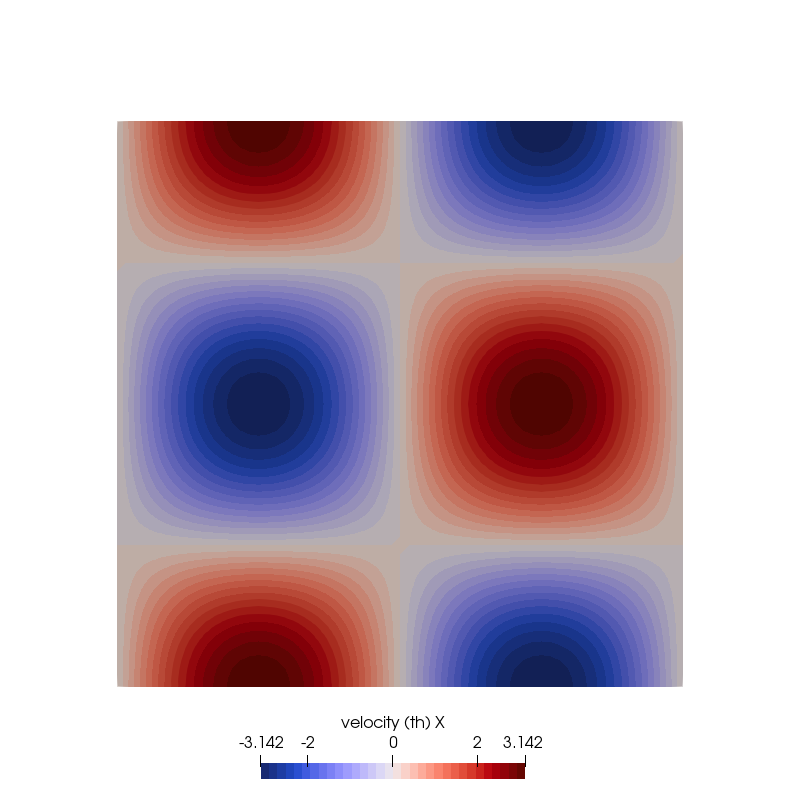
\includegraphics[width=3.74cm]{python_codes/fieldstone_32/results/u_1x1}
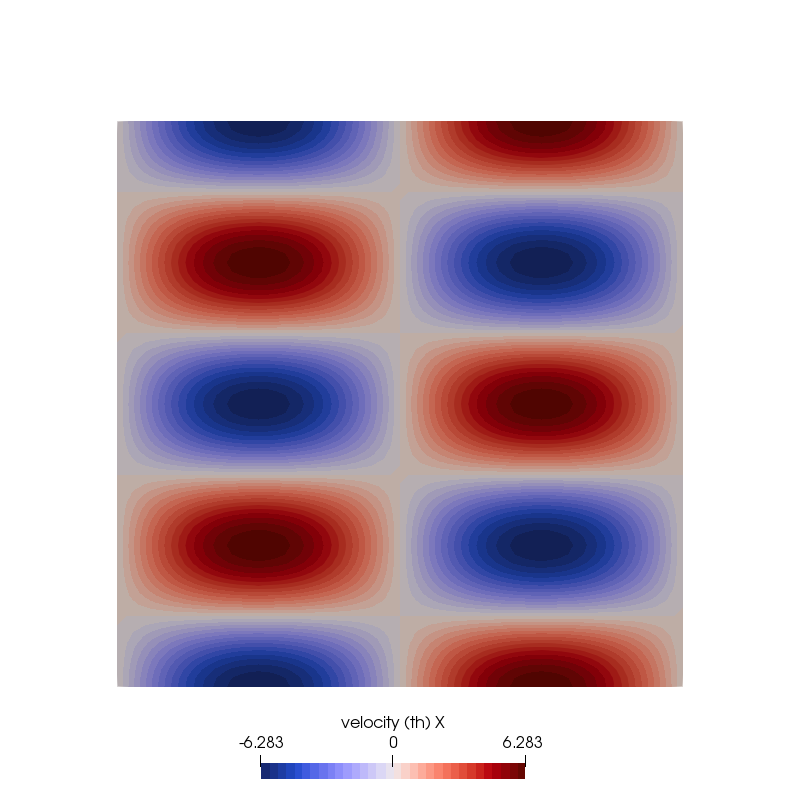
\includegraphics[width=3.74cm]{python_codes/fieldstone_32/results/u_1x2}
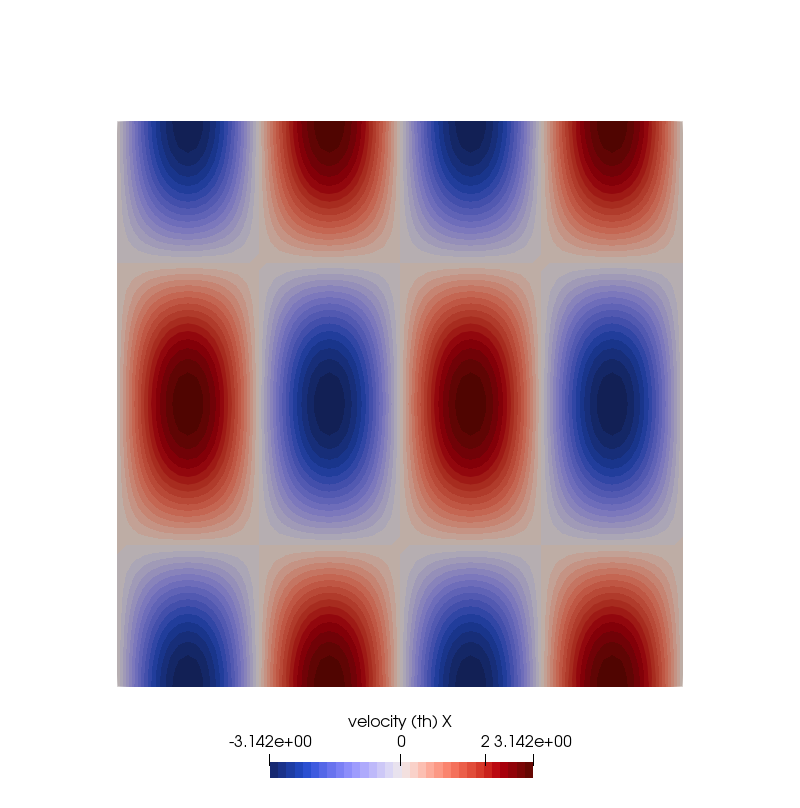
\includegraphics[width=3.74cm]{python_codes/fieldstone_32/results/u_2x1}
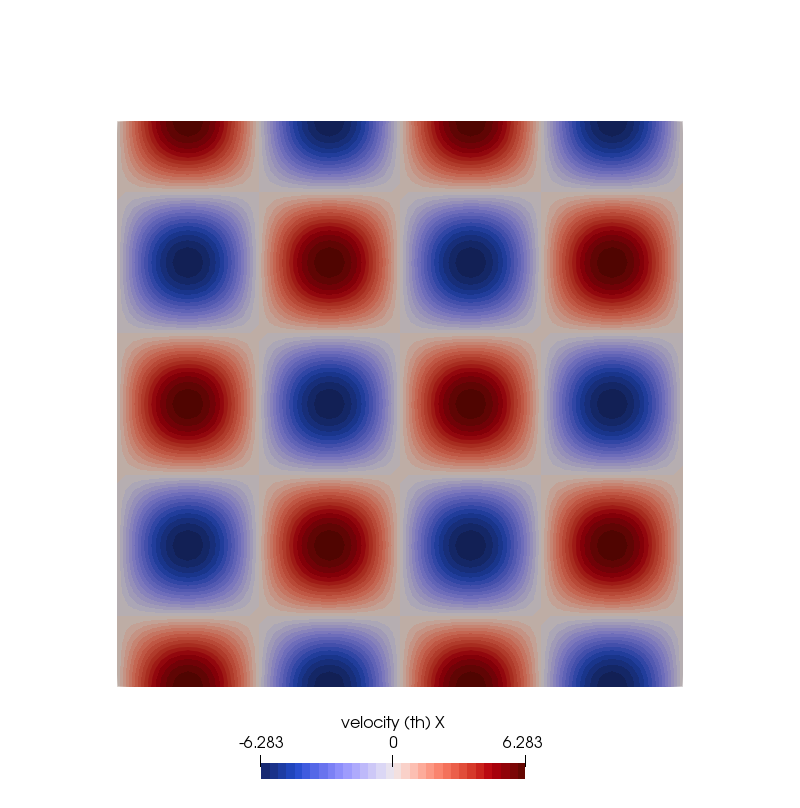
\includegraphics[width=3.74cm]{python_codes/fieldstone_32/results/u_2x2}\\
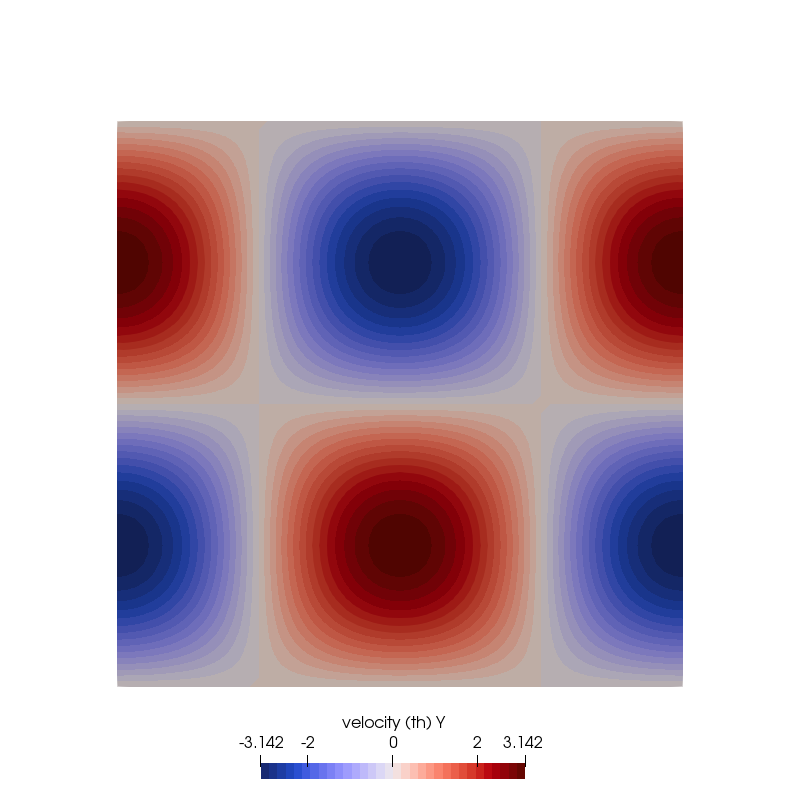
\includegraphics[width=3.74cm]{python_codes/fieldstone_32/results/v_1x1}
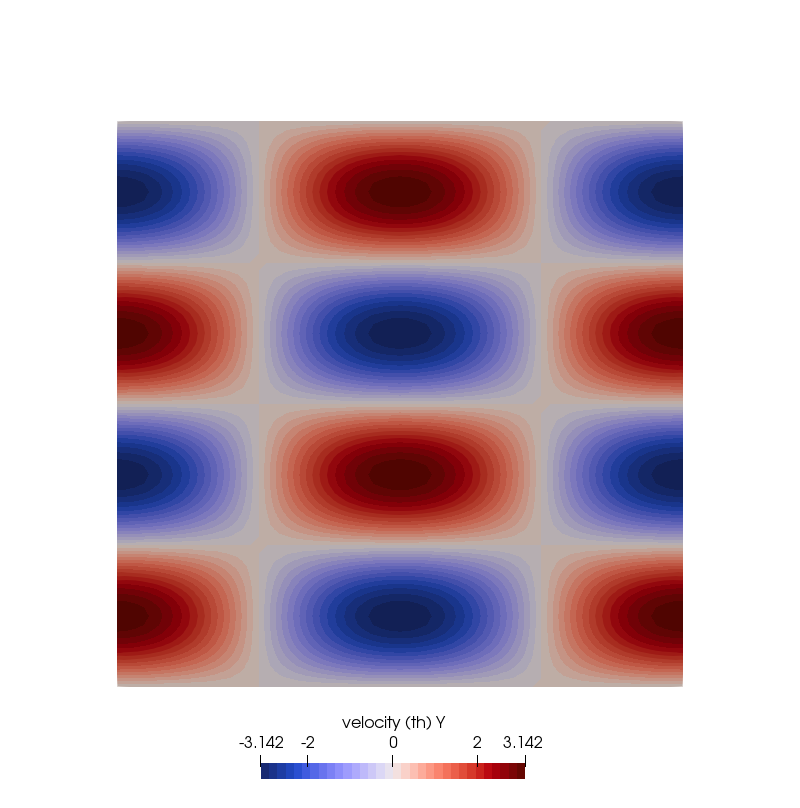
\includegraphics[width=3.74cm]{python_codes/fieldstone_32/results/v_1x2}
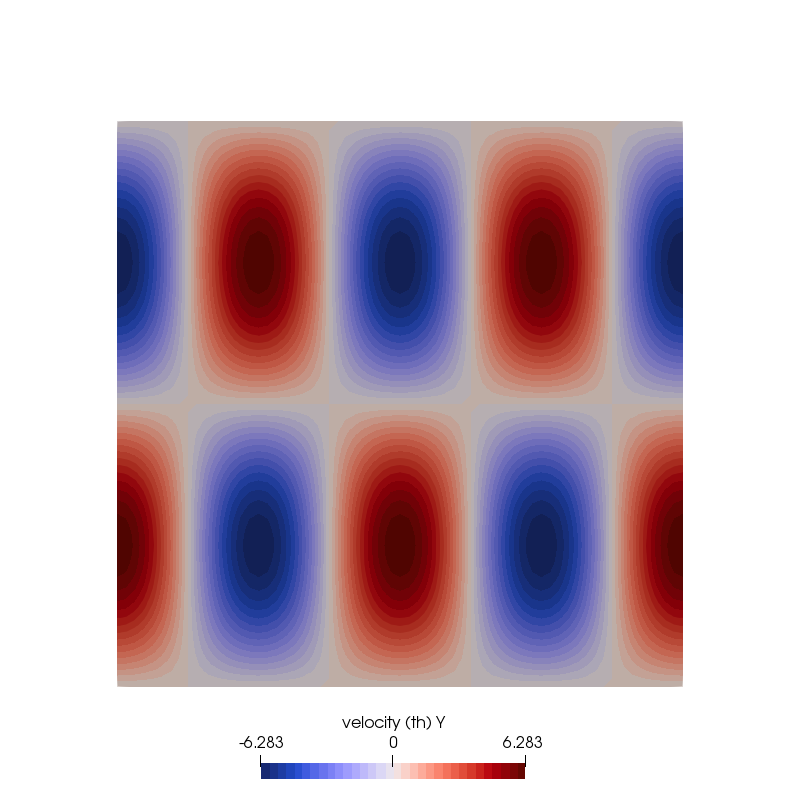
\includegraphics[width=3.74cm]{python_codes/fieldstone_32/results/v_2x1}
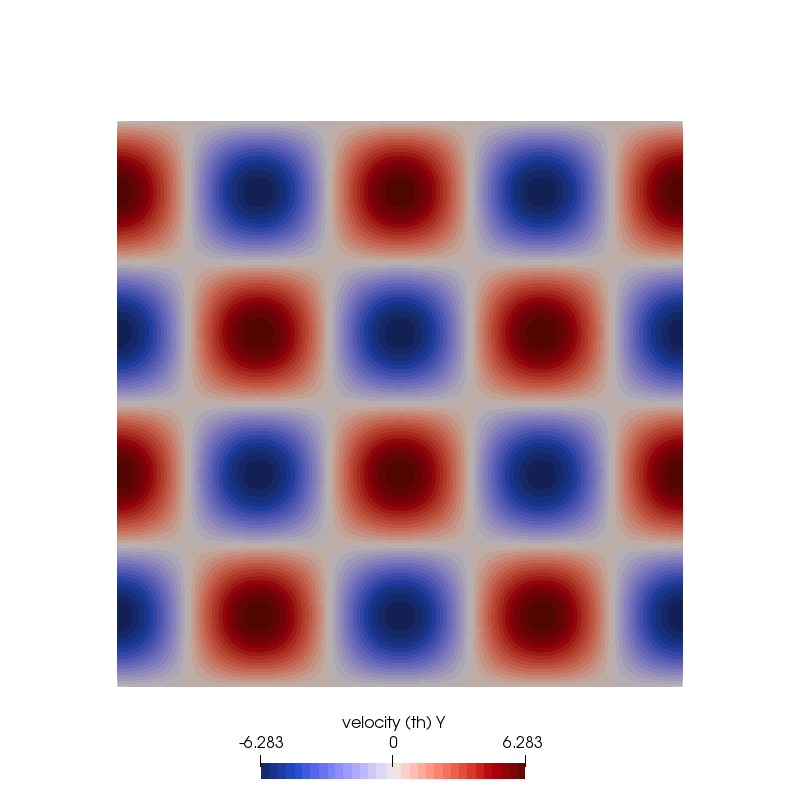
\includegraphics[width=3.74cm]{python_codes/fieldstone_32/results/v_2x2}\\
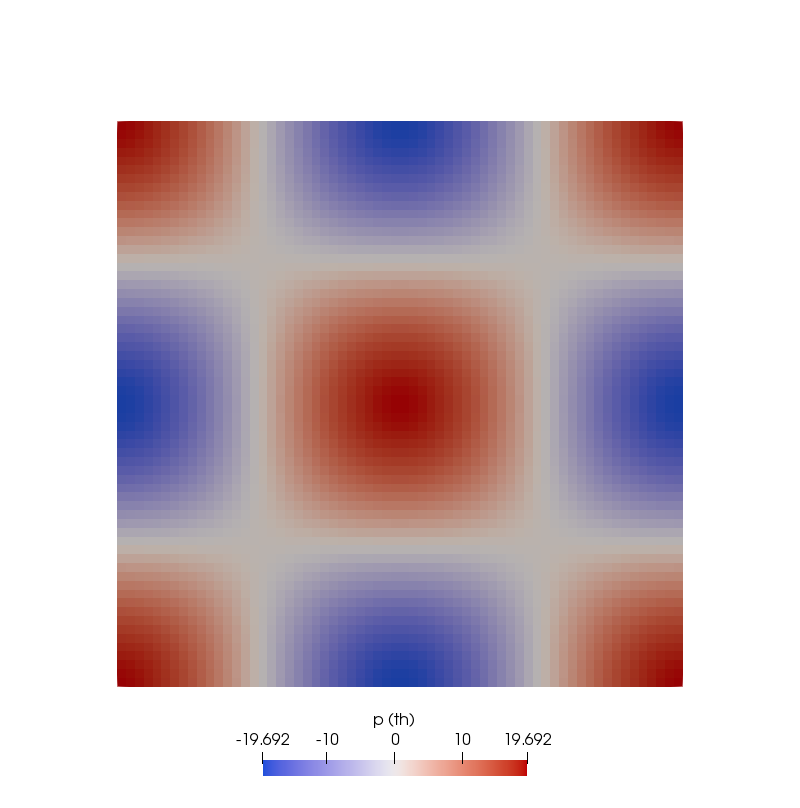
\includegraphics[width=3.74cm]{python_codes/fieldstone_32/results/p_1x1}
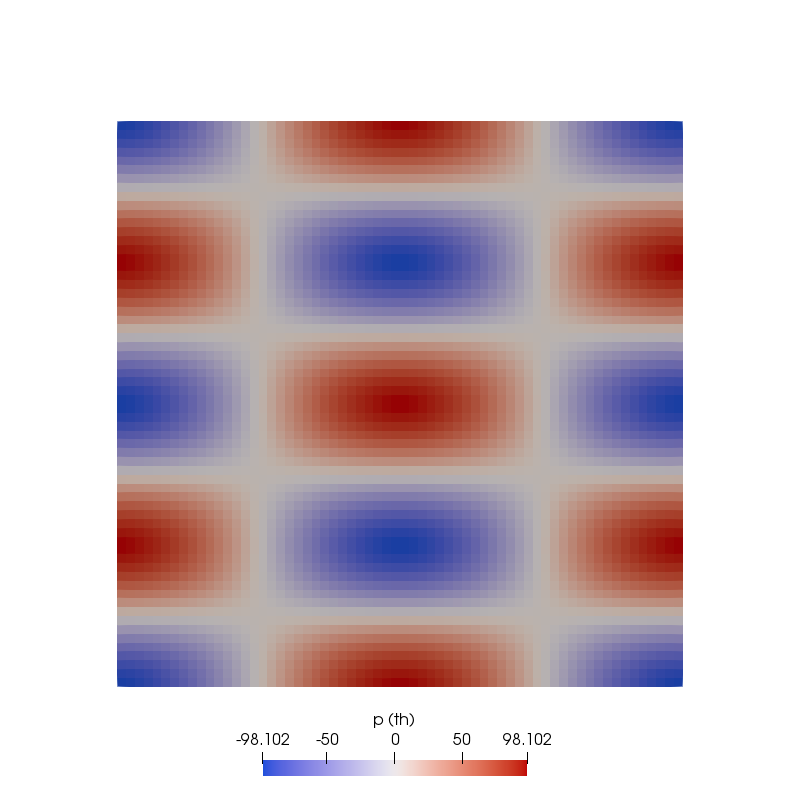
\includegraphics[width=3.74cm]{python_codes/fieldstone_32/results/p_1x2}
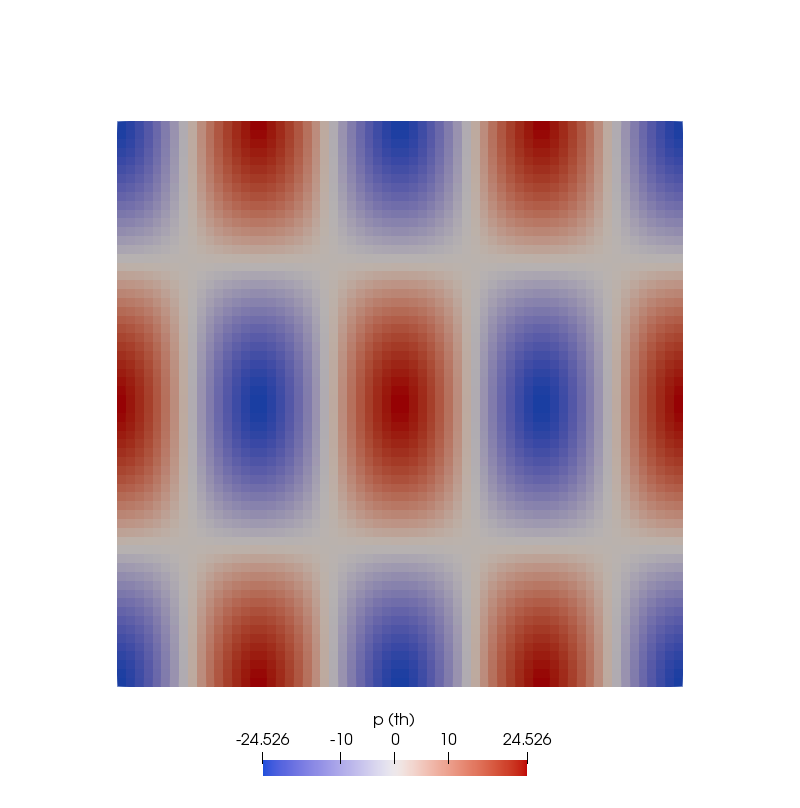
\includegraphics[width=3.74cm]{python_codes/fieldstone_32/results/p_2x1}
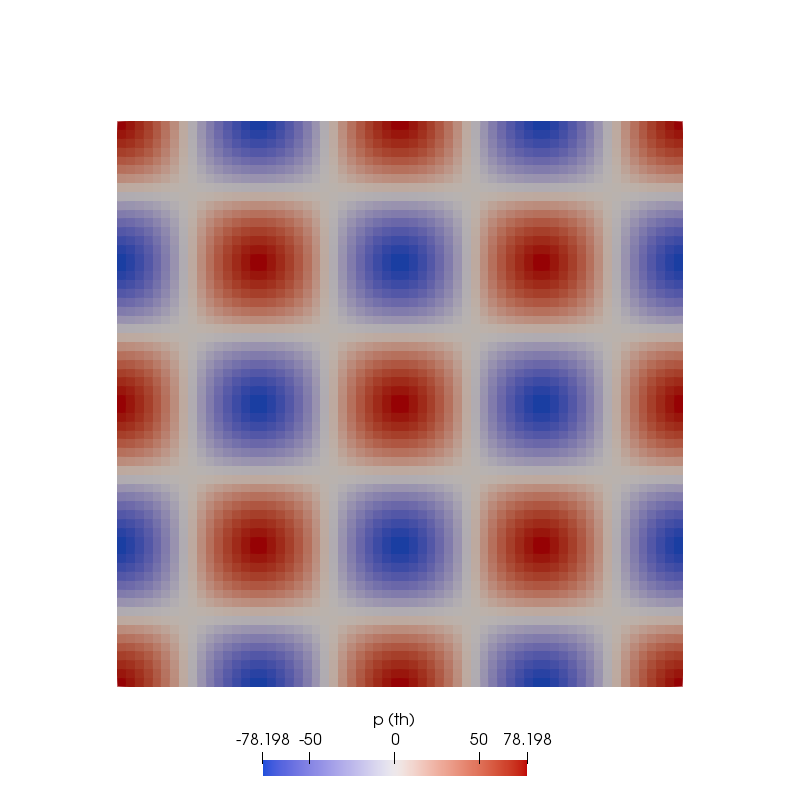
\includegraphics[width=3.74cm]{python_codes/fieldstone_32/results/p_2x2}\\
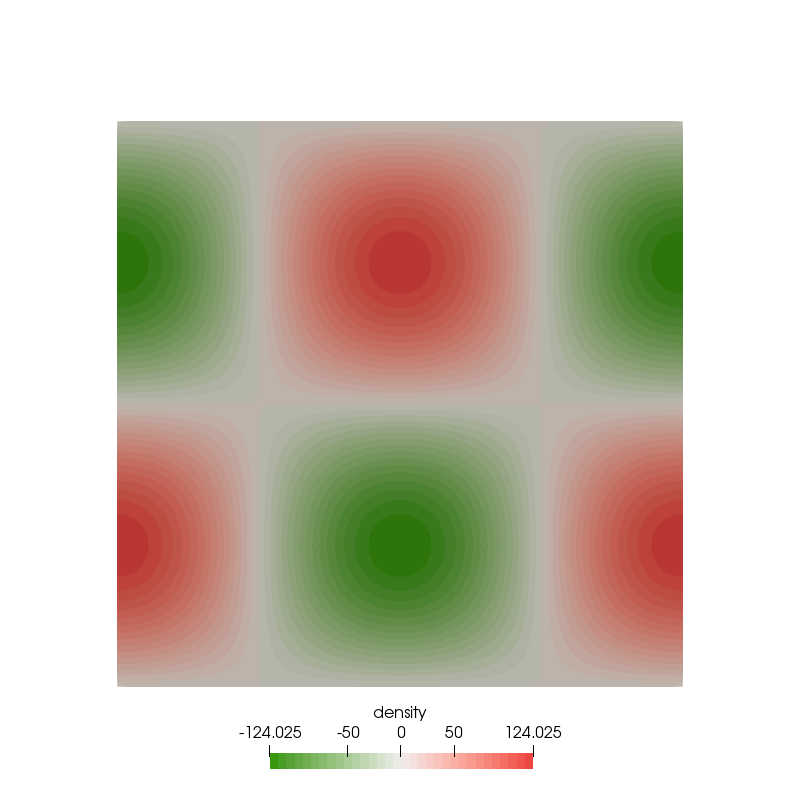
\includegraphics[width=3.74cm]{python_codes/fieldstone_32/results/rho_1x1}
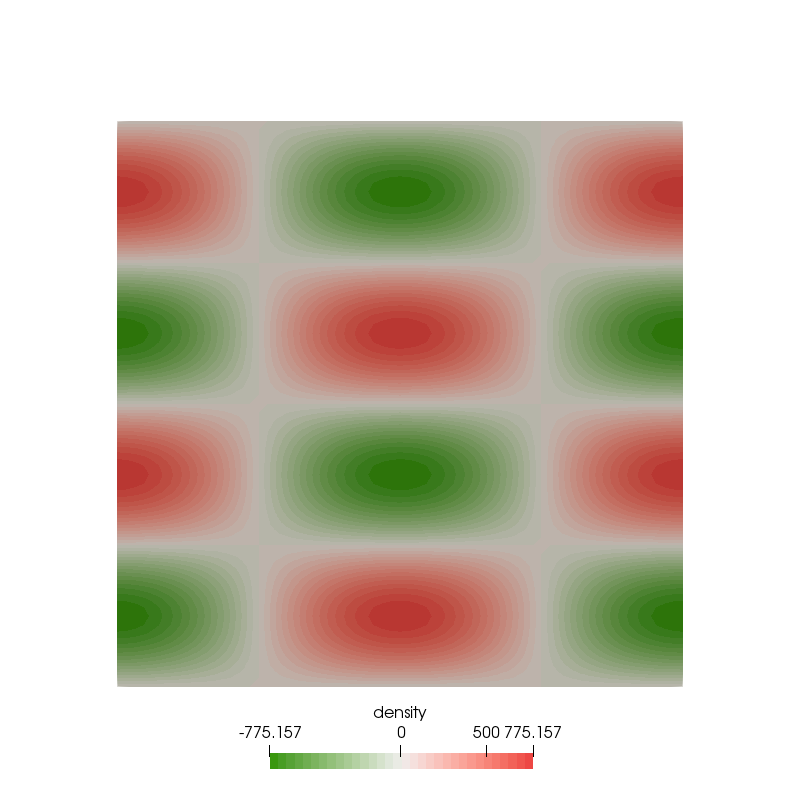
\includegraphics[width=3.74cm]{python_codes/fieldstone_32/results/rho_1x2}
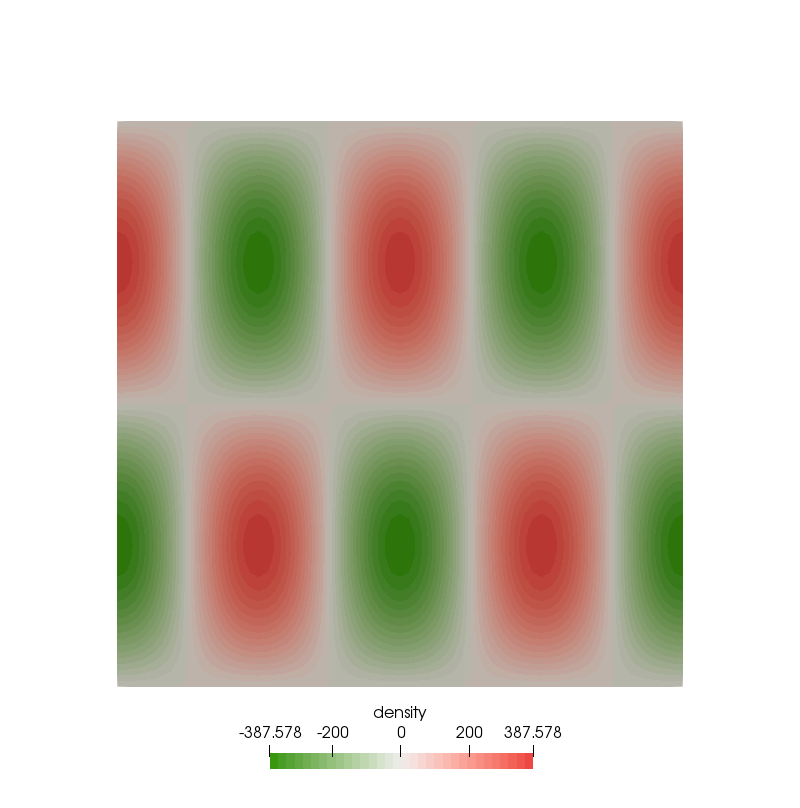
\includegraphics[width=3.74cm]{python_codes/fieldstone_32/results/rho_2x1}
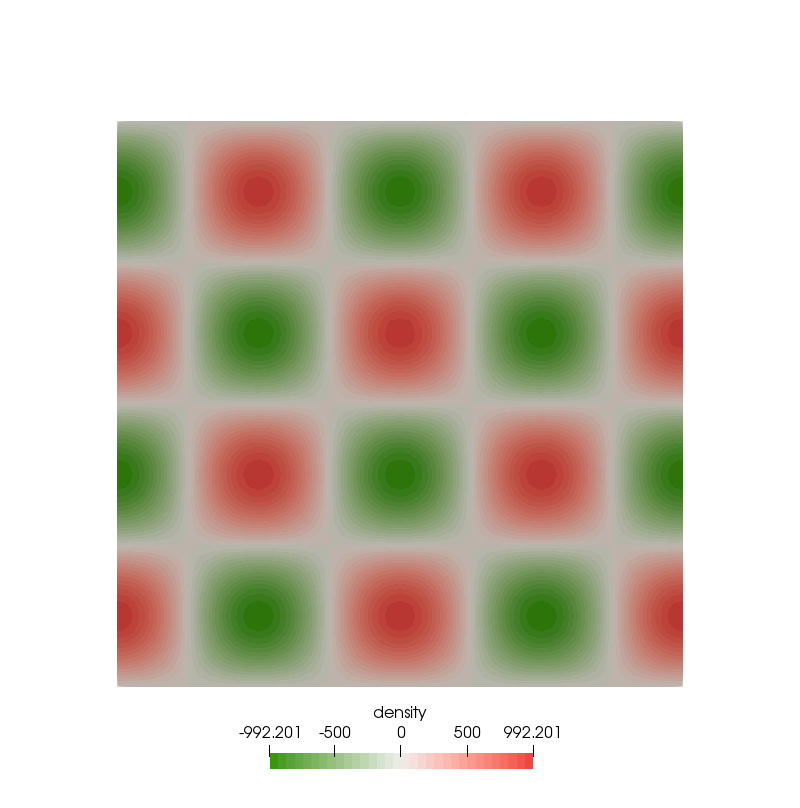
\includegraphics[width=3.74cm]{python_codes/fieldstone_32/results/rho_2x2}\\
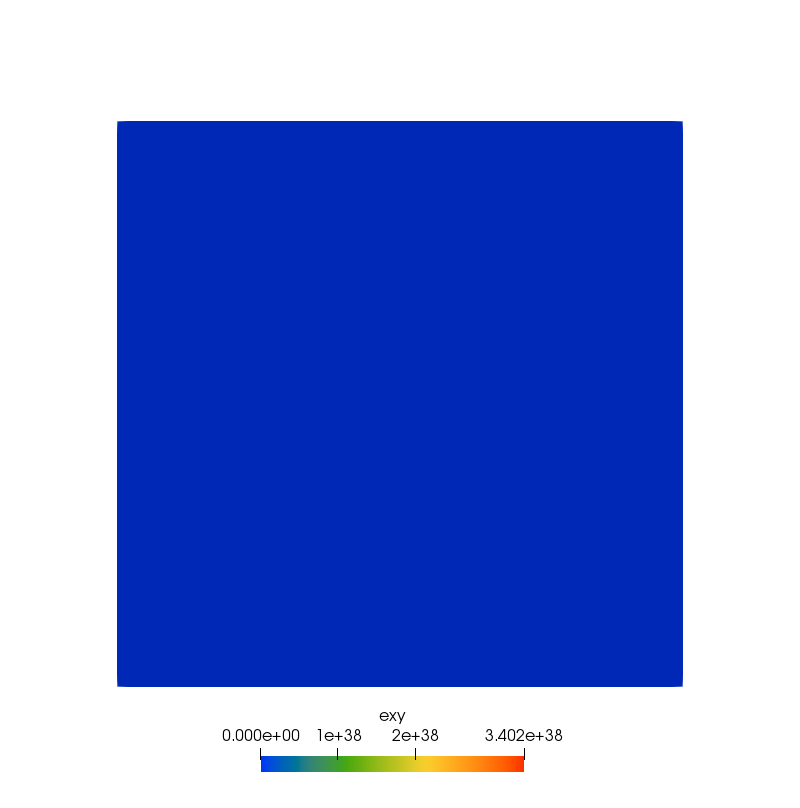
\includegraphics[width=3.74cm]{python_codes/fieldstone_32/results/exy_1x1}
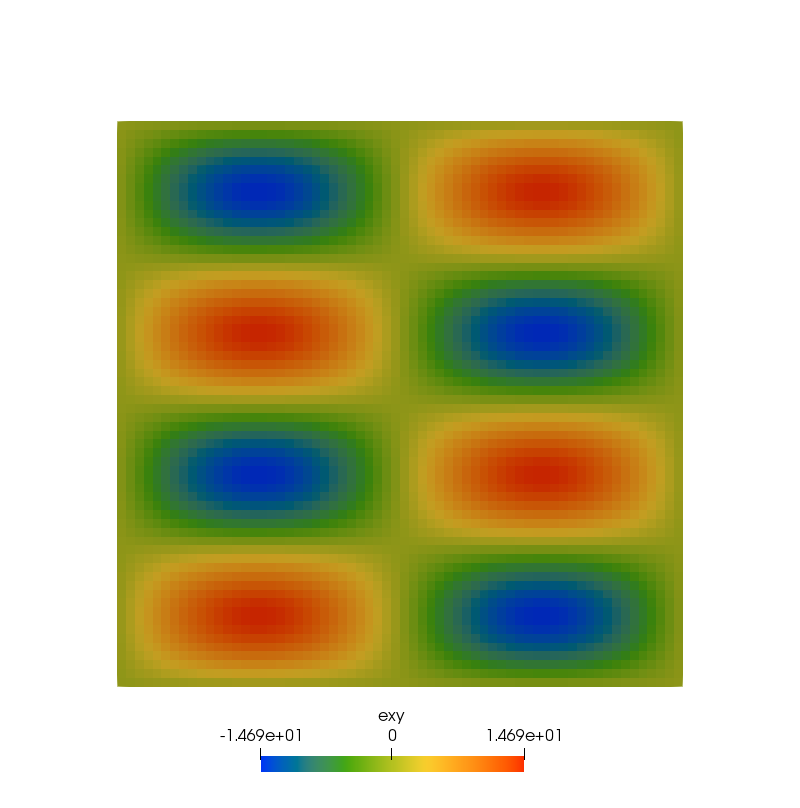
\includegraphics[width=3.74cm]{python_codes/fieldstone_32/results/exy_1x2}
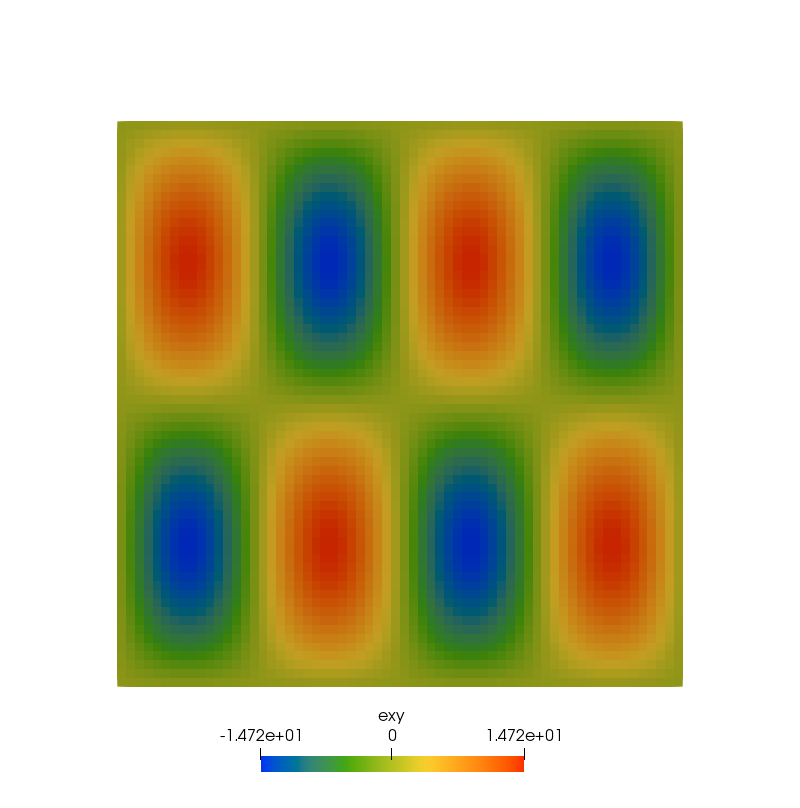
\includegraphics[width=3.74cm]{python_codes/fieldstone_32/results/exy_2x1}
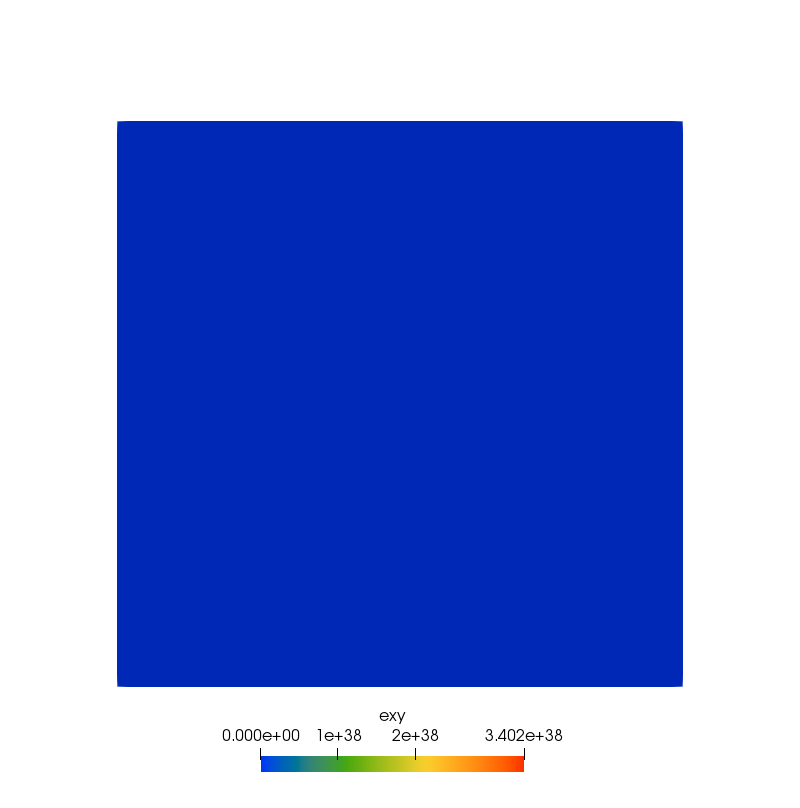
\includegraphics[width=3.74cm]{python_codes/fieldstone_32/results/exy_2x2}\\
{\small Top to bottom: Velocity components $u$ and $v$, pressure $p$, density $\rho$ and 
strain rate $\dot \varepsilon_{xy}$. 
From left to right: $(m,n)=(1,1)$, $(m,n)=(1,2)$, $(m,n)=(2,1)$, $(m,n)=(2,2)$ }
\end{center}

\newpage
\begin{center}
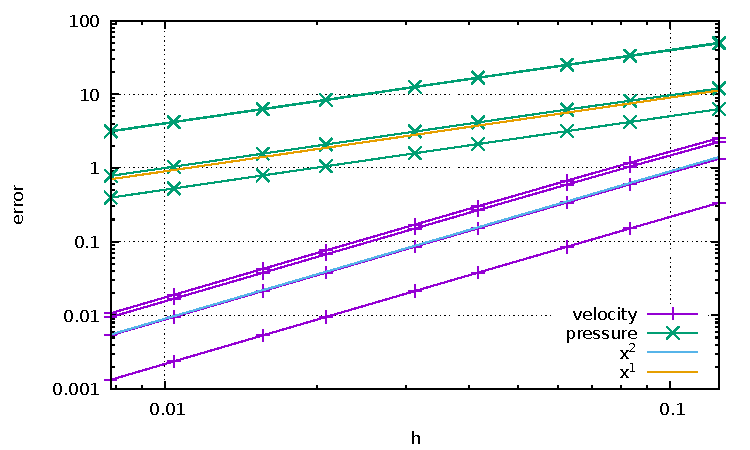
\includegraphics[width=11cm]{python_codes/fieldstone_32/results/errors}\\
{\small Errors for velocity and pressure for $(m,n)=(1,1),(1,2),(2,1),(2,2)$ }
\end{center}


\begin{center}
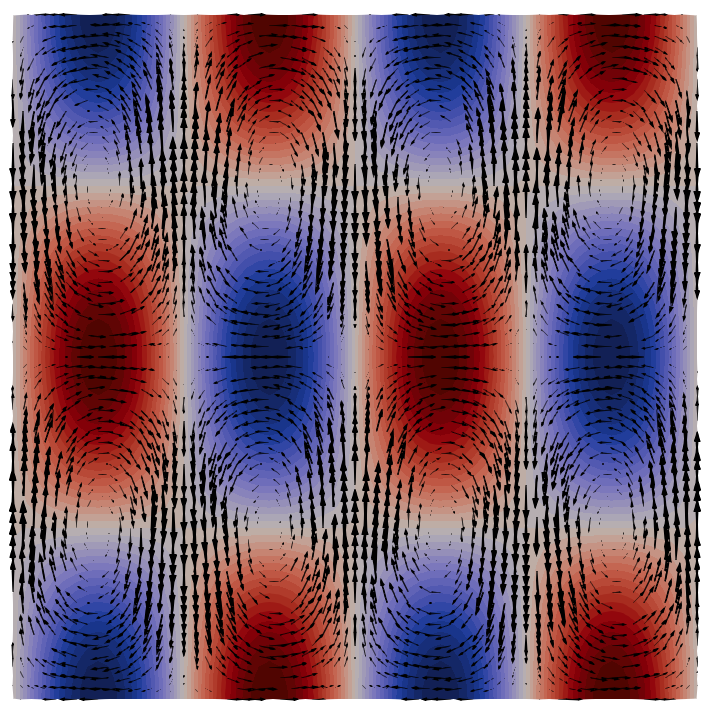
\includegraphics[width=14cm]{python_codes/fieldstone_32/results/vel_2x1}\\
{\small Velocity arrows for $(m,n)=(2,1)$}
\end{center}
